\section{Human validation of ProQuest candidates}
\subsection{Sampling and reviewer provenance}
Two human reviewers evaluated the same 300 claims from 299 distinct articles: 250 historical claims and 50 from the modern extension. The author confirmed the first review was completed without AI assistance on October 21, and confirmed both reviewers were human on October 22. Reviewer 2's frozen labels and dated author attestation are preserved separately. The second review protocol records source-only reading without consulting claim-level author labels, machine labels, or realized outcomes; aggregate study summaries had been visible. The first review had mixed machine-label exposure, as detailed below. Inter-reviewer agreement and adjudication have not yet been performed; two completed reviews do not imply a fully blinded design.\evidence{V1--V3}

The original historical batch contains 150 claims from a frame of 175,843 scored verified candidates after excluding 12 pilot records. It retains an initial simple random sample of 100 and adds 50 without replacement from the remaining frame. The initial 100 had prior machine-label exposure; the additional 50 are documented as having machine labels hidden until the annotation was frozen. The second historical batch samples another 100 without replacement from 175,693 remaining eligible addresses. Its findings are shown separately rather than presenting the entire review as an untouched blinded experiment.

The modern batch is stratified by publication year: four records from each of 2011 and 2026 and three from each intervening year. Its frame contains 91,118 retained verified candidates and includes verification exceptions that the predictive analysis later excludes. Unlike the historical frame, these records need not have scorable outcomes. Differences in sample design and eligibility prevent interpreting the pooled 300-record inclusion fraction as a single population validity estimate.

\begin{table}[t]
\caption{First-reviewer inclusion decisions by review batch}\label{tab:review}
\centering\small
\begin{tabularx}{\linewidth}{Xrrrr}
\toprule
Sample & Reviewed & Include & Exclude & Unclear\\
\midrule
Historical batch 1 & 150 & 105 & 44 & 1\\
Historical batch 2 & 100 & 72 & 28 & 0\\
Modern extension & 50 & 35 & 15 & 0\\
\midrule
Reviewed sample total & 300 & 212 & 87 & 1\\
\bottomrule
\end{tabularx}
\note{The total is a record count across different frames, not a pooled population estimate. Historical batches are positive candidates already eligible for legacy scoring; modern sampling covers all retained candidates by year. Source recovery succeeded for sampled records, with documented lineage checks. Sources: V1--V2.}
\end{table}

Inclusion is 105/150 in the original historical batch and 72/100 in the second. The unresolved first-batch case gives a 70.0--70.7\% identification range depending on how that case is classified; this is not a confidence interval. The modern sample includes 35/50 candidates. The saved inverse-inclusion-probability ratio estimate is 73.4\% for its modern frame, versus the unweighted 70.0\% sample fraction. No design-based interval is supplied for that weighted point estimate, and none is invented here.

Reviewer 2 includes 171 of the 250 historical candidates and excludes 79; among the 50 modern candidates, 33 are included and 17 excluded. The second review therefore contains 204 include and 96 exclude decisions. These are descriptive counts from the frozen manifest, not an agreement calculation: matching aggregate counts would not establish that reviewers accepted the same claims. The two sets of judgments remain separate, with no adjudicated consensus or second-reviewer population-weighted estimate asserted here.\evidence{V3}

\subsection{Field agreement and practical usability}
The field-agreement results below compare machine labels with the first human reviewer and are conditional on that reviewer's inclusion decisions. They are not human--human agreement estimates. Table~\ref{tab:fields} reports exact numerator and denominator pairs, because excluding invalid candidates changes the population to which the field rates apply. The historical review shows stronger topic and direction agreement than horizon and scope agreement. In the modern included subset, topic and direction each match on 29/35 claims, horizon on 26/35, and scope on 24/35. These comparisons support using the extraction to organize candidate material, but also identify consequential interpretation errors.

\begin{table}[t]
\caption{Machine--first-reviewer field agreement among included claims}\label{tab:fields}
\centering\small
\begin{tabularx}{\linewidth}{Xrrr}
\toprule
Field & Historical 1 & Historical 2 & Modern\\
\midrule
Topic & 90/105 (85.7\%) & 66/72 (91.7\%) & 29/35 (82.9\%)\\
Direction & 94/105 (89.5\%) & 60/72 (83.3\%) & 29/35 (82.9\%)\\
Horizon & 66/105 (62.9\%) & 49/72 (68.1\%) & 26/35 (74.3\%)\\
Scope & 65/105 (61.9\%) & 49/72 (68.1\%) & 24/35 (68.6\%)\\
Confidence & 75/105 (71.4\%) & 55/72 (76.4\%) & 22/35 (62.9\%)\\
Voice & 79/105 (75.2\%) & 57/72 (79.2\%) & 24/35 (68.6\%)\\
Speaker name & 74/105 (70.5\%) & 43/72 (59.7\%) & 27/35 (77.1\%)\\
\bottomrule
\end{tabularx}
\note{Literal agreement is not always semantic equivalence: name abbreviations can count as mismatches. These are sample summaries, without claimed independent-observation confidence intervals. Current-state agreement is excluded because the original batch used incompatible conventions. Sources: V1--V2.}
\end{table}

\begin{figure}[t]
\centering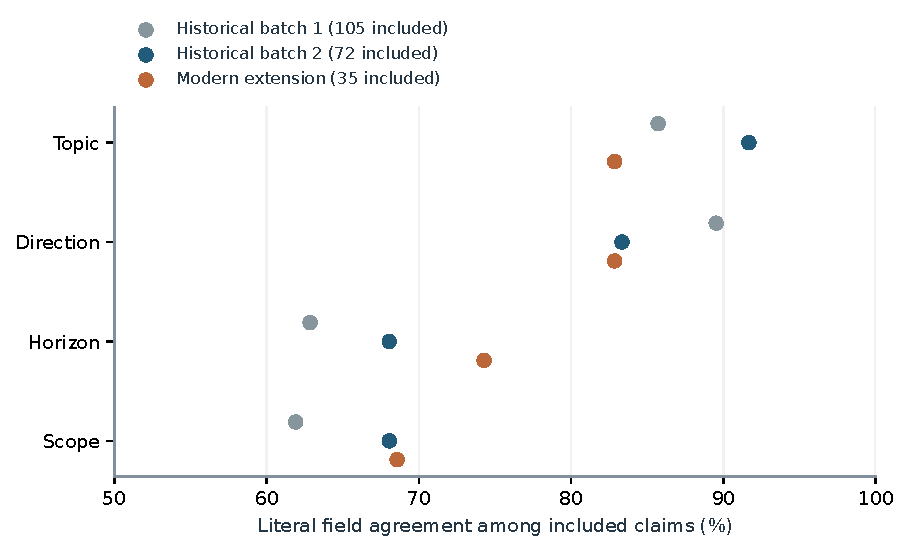
\includegraphics[width=.95\linewidth]{human_agreement.pdf}
\caption{Machine--first-reviewer agreement varies by field and review batch. Displaying the three samples separately preserves their different frames and denominators. Small differences between samples should not be read as statistically established changes over time.}\label{fig:human}
\end{figure}

Several conventions limit interpretation. The review maps approximately four to eight months to six and nine to fifteen months to twelve; annual next-year outlooks also map to twelve. A matching horizon category therefore does not establish an exact endpoint. Speaker-name comparison is literal, so a surname and a full name can disagree while referring to the same person. Price and unemployment fields contain many not-applicable matches; the additional review's applicable-only counts are 12/14 and 4/6, respectively, and are too small to characterize performance broadly.

The original current-state field cannot be pooled with the additional batch. Its saved mismatch reflects differing coding conventions, and the all-eleven-fields match count of 1/105 is consequently not a valid overall accuracy estimate. In the additional batch, all eleven fields match on 6/107 included claims, but even that is exact annotation agreement, not the share of forecasts whose economic outcomes are scored correctly. Joint usability must be defined by the fields needed for a particular estimand, rather than requiring or ignoring fields indiscriminately.

\subsection{What the audit validates}
Four quantities must remain distinct. Inclusion measures whether a proposed passage is a forecast under the review rubric. Field agreement measures whether a retained forecast's annotations match the review. Recall measures whether all genuine forecasts in a document were found. Economic accuracy measures whether a forecast matches its eventual outcome under a specified interpretation. The human sample estimates aspects of the first two; it does not establish the third, and its purpose is not to estimate the fourth.

The review identifies practical error categories: present or past descriptions treated as forecasts, unresolved policy conditionals, generic statements, ambiguous attribution, coarse horizons, and mismatches between geographic scope and the proposed benchmark. The categorical local exports do not provide a consistently coded frequency table for these categories. We therefore discuss them qualitatively and do not invent prevalence estimates or quote restricted source prose. Appendix~\ref{app:examples} supplies explicitly hypothetical examples to clarify the distinctions.

Most importantly, the review does not produce a source-validated strict score for the full corpus. Such a score would require the exact economic quantity, direction, scope, original date, conditionality, and endpoint to be compatible with the outcome rule. The historical estimates below remain estimates for machine-selected, machine-labeled candidates. A global correction using the pooled inclusion fraction would be unjustified because extraction errors can vary with topic, era, horizon, and realized outcome.

